\subsection{Case04 - Layer 3 forwarding	}
\label{xdp_wifi_case04}

En este caso de uso se explorará el forwarding de paquetes, en este punto ya se debe conocer como filtrar por las cabeceras de los paquetes, analizarlos y establecer una lógica asociada a ese filtrado con los códigos de retorno \gls{xdp}. La gran diferencia en este entorno inalámbrico es el número de interfaces que suele tener un dispositivo \textit{wireless}. Generalmente en entornos cableados, un nodo suele tener tantas interfaces Ethernet como enlaces tenga con otros nodos, en cambio, en entornos wireless, con una misma interfaz puede tener enlaces con otros nodos siempre y cuando se encuentren en rango.\\
\par
Por tanto, los programas \gls{xdp} en entornos inalámbricos podrían realizar todo su forwarding haciendo uso de un único código de retorno \gls{xdp}, \texttt{XDP\_TX}. Con dicho código se reenviarían los paquetes recibidos a la interfaz a la cual llegaron los paquetes. Dado que en los entornos cableados, se tuvieron que hacer uso de los \textit{helpers} \gls{bpf} indicados en el bloque \ref{code:case04_xdp_ether_kernprog1}, se van a plantear escenarios similares donde sea necesario hacer un forwarding de una interfaz A a otra B. De esta forma, se verificará que dichas funciones siguen operativas en interfaces creadas con el módulo mac80211\_hwsim.\\
\par
No se ha querido plantear este caso de uso haciendo solo uso  del código de retorno \texttt{XDP\_TX}, ya que en el case03 \gls{xdp} \textit{Wireless} (Ir a \ref{xdp_wifi_case03}),  ya se hizo uso de este código y se vio que funcionaba correctamente, por lo que se entendía que era preferible explorar los \textit{helpers} \gls{bpf} en entornos inalámbricos.
 


\vspace{0.5cm}
\textbf{Compilación}\\
\par

Para compilar el programa \gls{xdp}, al igual que en casos de uso anteriores, se ha dejado un Makefile preparado en este directorio. Por lo tanto, para compilarlo únicamente hay que seguir las indicaciones del bloque \ref{code:case04_xdp_wifi_compilacion}.

\begin{lstlisting}[language= bash, style=Consola, caption={Compilación programa XDP - Case04},label=code:case04_xdp_wifi_compilacion]
    # En caso de no haber entrado en el directorio asignado del caso de uso
    cd TFG/src/use_cases/xdp-wireless/case04
    
    
    # Hacemos uso del Makefile suministrado 
    sudo make
\end{lstlisting}
\vspace{0.5cm}

Si tiene dudas sobre el proceso de compilación del programa \gls{xdp} le recomendamos que vuelva al case02 (\gls{xdp} - Cableado \ref{xdp_ether_case02}) donde se hace referencia al \textit{flow} dispuesto para la compilación de los programas \gls{xdp}.\\
\par



\vspace{0.5cm}
\textbf{Puesta en marcha del escenario}\\
\par

Para testear los programas \gls{xdp} en un entorno inalámbrico, se hará uso de Mininet-WiFi para emular las topologías de red. Para levantar el escenario solo se tendrá que ejecutar el script en Python que hace uso de la API de Mininet-WiFi para generar toda la topología de red. Una vez ejecutado este abrirá la interfaz de linea de comandos de Mininet-WiFi, desde la cual se podrá comprobar el funcionamiento del caso de uso. \\
\par

Para limpiar la máquina del escenario recreado anteriormente con Mininet-WiFi se podría realizar un \texttt{sudo mn -c}, pero se recomienda al usuario que haga uso del \textit{target} del Makefile destinado para ello, ya que adicionalmente limpiará los ficheros intermedios generados en el proceso de compilación de nuestro programa \gls{xdp}. Ejecutando el siguiente comando se limpiaría la máquina.

\begin{lstlisting}[language= bash, style=Consola, caption={Compilación programa XDP - Case04},label=code:case04_xdp_wifi_run]
    # Levantamos el escenario
    sudo python runenv.py
      
    # Limpiamos el escenario
    sudo make clean
\end{lstlisting}
\vspace{0.5cm}

%%%%%%%%%%%%%%%%%%%%%%%%%%%%%%%%%%%%%%%%%%%%%%%%%%%%%%%%%%%%%%%%%%%%%%%%%%%%%%%%%%%%
\subsubsection{Hardcoded forwarding}
\label{xdp_wifi_case04_hard}

La primera forma de implementación del forwarding es lo que denominaremos como Hardcoded forwarding. Como ya se comentó, es necesario hardcodear información de forwarding en el propio programa \gls{xdp}. El escenario levantado (Ver figura \ref{fig:case04_xdp_wifi_scenario}), está compuesto de una estación wireless y un host, que corren dentro de su respectivas \textit{Network Namespaces}, y un punto de acceso corriendo un proceso de HostApd para comunicar las dos estaciones wireless entre sí. De forma adicional, y por consistencia del caso de uso, se ha decidido correr dicho switch dentro de su propia \textit{Network Namespace} para que no haya lugar a dudas de que el forwarding se está realizando correctamente y no está habiendo \textit{by-passes} de ningún tipo. En este caso el forwarding lo haremos desde la interfaz \texttt{ap1-wlan1} hacia la interfaz \texttt{ap1-eth2}.\\
\par

% figura escenario
\begin{figure}[ht]
    \centering
    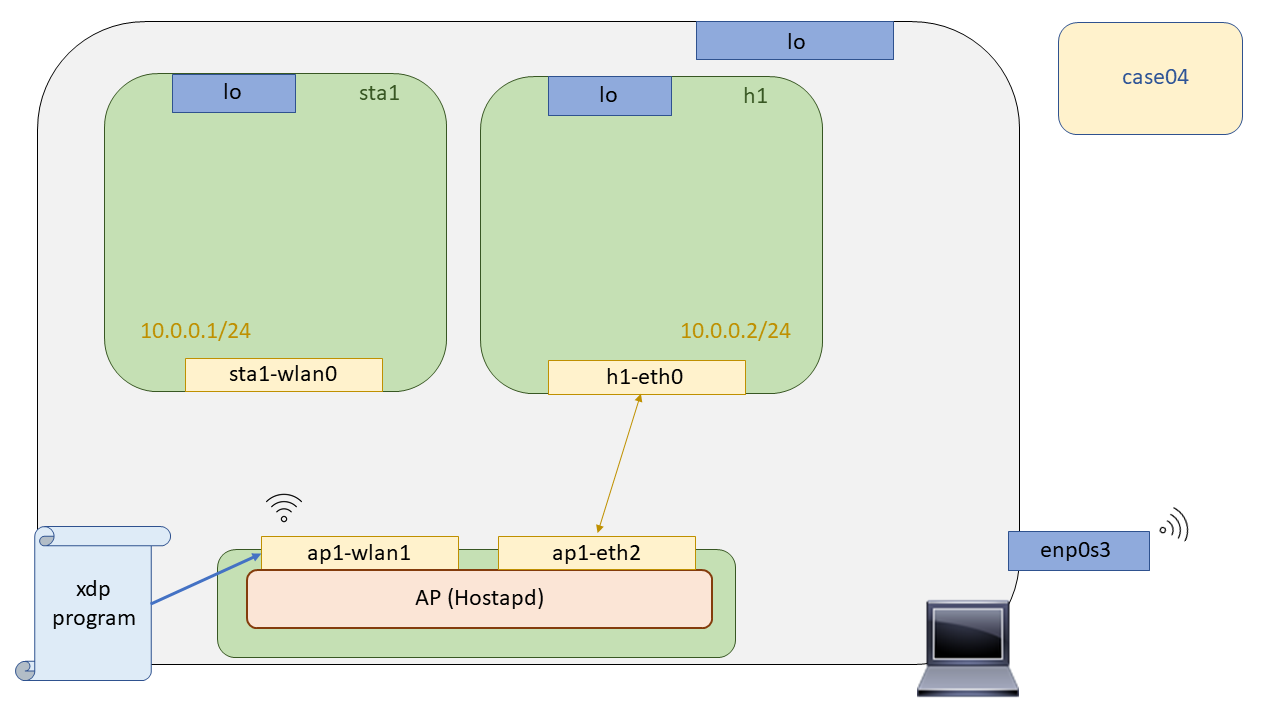
\includegraphics[width=14cm]{archivos/img/dev/xdp-wifi/case04/scenario.png}
    \caption{Escenario inalámbrico Hardcoded forwarding del Case04 - XDP}
    \label{fig:case04_xdp_wifi_scenario}
\end{figure}


\vspace{0.5cm}
\textbf{Carga del programa XDP}\\
\par

Antes de realizar la carga del programa se deben obtener dos datos, la \textit{ifindex} de la interfaz \texttt{ap1-eth2} a la cual se va a mandar los paquetes generados desde la estación wireless \texttt{sta1}. Y la MAC de la interfaz del host1, ya que será necesario que los paquetes que se dirijan a la interfaz \texttt{ap1-wlan1} lleven como MAC destino la de la \texttt{ap1-eth2} para que así los paquetes no sean descartados. \\
\par
Una vez se tengan estos datos anotados se abrirá el programa \gls{xdp} (\texttt{*.c}) cuan cualquier editor de texto,  se irá a la declaración de variables y se hardcodeará tanto el \textit{ifindex} como la MAC. Véase un ejemplo en el bloque \ref{code:case04_xdp_ether_kernprog2}.\\
\par

Una vez que se tenga hardcodeado los datos para realizar el forwarding se deberá recompilar el programa \gls{xdp} para que el \textit{bytecode} que se ancle a la interfaz \texttt{ap1-wlan1} haga correctamente el forwarding. Por ello, simplemente se tiene que hacer un \texttt{make} nuevamente. Ahora sí, ya se tiene todo preparado para anclar de nuevo el programa \gls{xdp}. En este caso la carga del programa \gls{xdp} se llevará a cabo una vez levantado el escenario vía CLI de Mininet-WiFi como se puede apreciar en el bloque \ref{code:case04_xdp_wifi_load1}.

\begin{lstlisting}[language= bash, style=Consola, caption={Carga del programa XDP Hardcoded forwarding - Case04},label=code:case04_xdp_wifi_load1]
    # Antes que nada, debemos lanzar el escenario en caso de que no lo hayamos hecho todavía.
    sudo python runenv.py
    
    
    # Ejecutamos el siguiente comando dentro de la Network Namespace del AP1, cargando así el
    # programa XDP en la interfaz ap1-wlan1.
    mininet-wifi> ap1 ./xdp_loader -d ap1-wlan1 -F --progsec xdp_case04 -S
\end{lstlisting}

\vspace{0.7cm}
\textbf{Comprobación del funcionamiento}\\
\par

La comprobación de funcionamiento de este programa \gls{xdp} es bastante básica: se van a generar paquetes desde la estación \textit{wireless} \texttt{sta1} hacia el host, \texttt{h1}. Para ello se abrirán dos terminales, en cada una de ellas se llevará a cabo una tarea.

\begin{lstlisting}[language= bash, style=Consola, caption={Comprobación del funcionamiento Hardcoded forwarding - Case04},label=code:case04_xdp_wifi_func1]
    # Abrimos las dos terminales
    mininet-wifi> xterm h1 sta1
    
    # En la terminal del host1 pondremos a un sniffer a escuchar los paquetes que nos lleguen.
    [Terminal:h1] tcpdump -l
    
    # En la terminal de la sta1 lanzaremos pings contra el h1
    [Terminal:sta1] ping 10.0.0.2
    
    # Por último, opcionalmente, podemos ejecutar el programa que actuaba como recolector de estadísticas sobre los códigos de retorno XDP
    mininet-wifi> ap1 ./xdp_stats -d ap1-wlan1
\end{lstlisting}

Atendiendo a la figura \ref{fig:case04_xdp_wifi_func1}, se puede ver como el ping \fcolorbox{black}{ProcessBlue}{\rule{0pt}{2.5pt}\rule{2.5pt}{0pt}}\hspace{1mm} no funciona, y podría surgir la siguiente pregunta, ¿por qué no hay conectividad? No es que el programa no funcione, lo que sucede es que la comunicación actualmente solo está soportada en un sentido, ya que solo se está soportando el forwarding de la interfaz \texttt{ap1-wlan1} a la interfaz \texttt{ap1-eth2}. Actualmente el proceso de ping está detenido en la resolución ARP de la MAC asociada a la dirección IP \texttt{10.0.0.2}, llegando los ARP-Request pero los ARP-Reply nunca llegarán a su destino.\\
\par

% figura escenario
\begin{figure}[ht!]
    \centering
    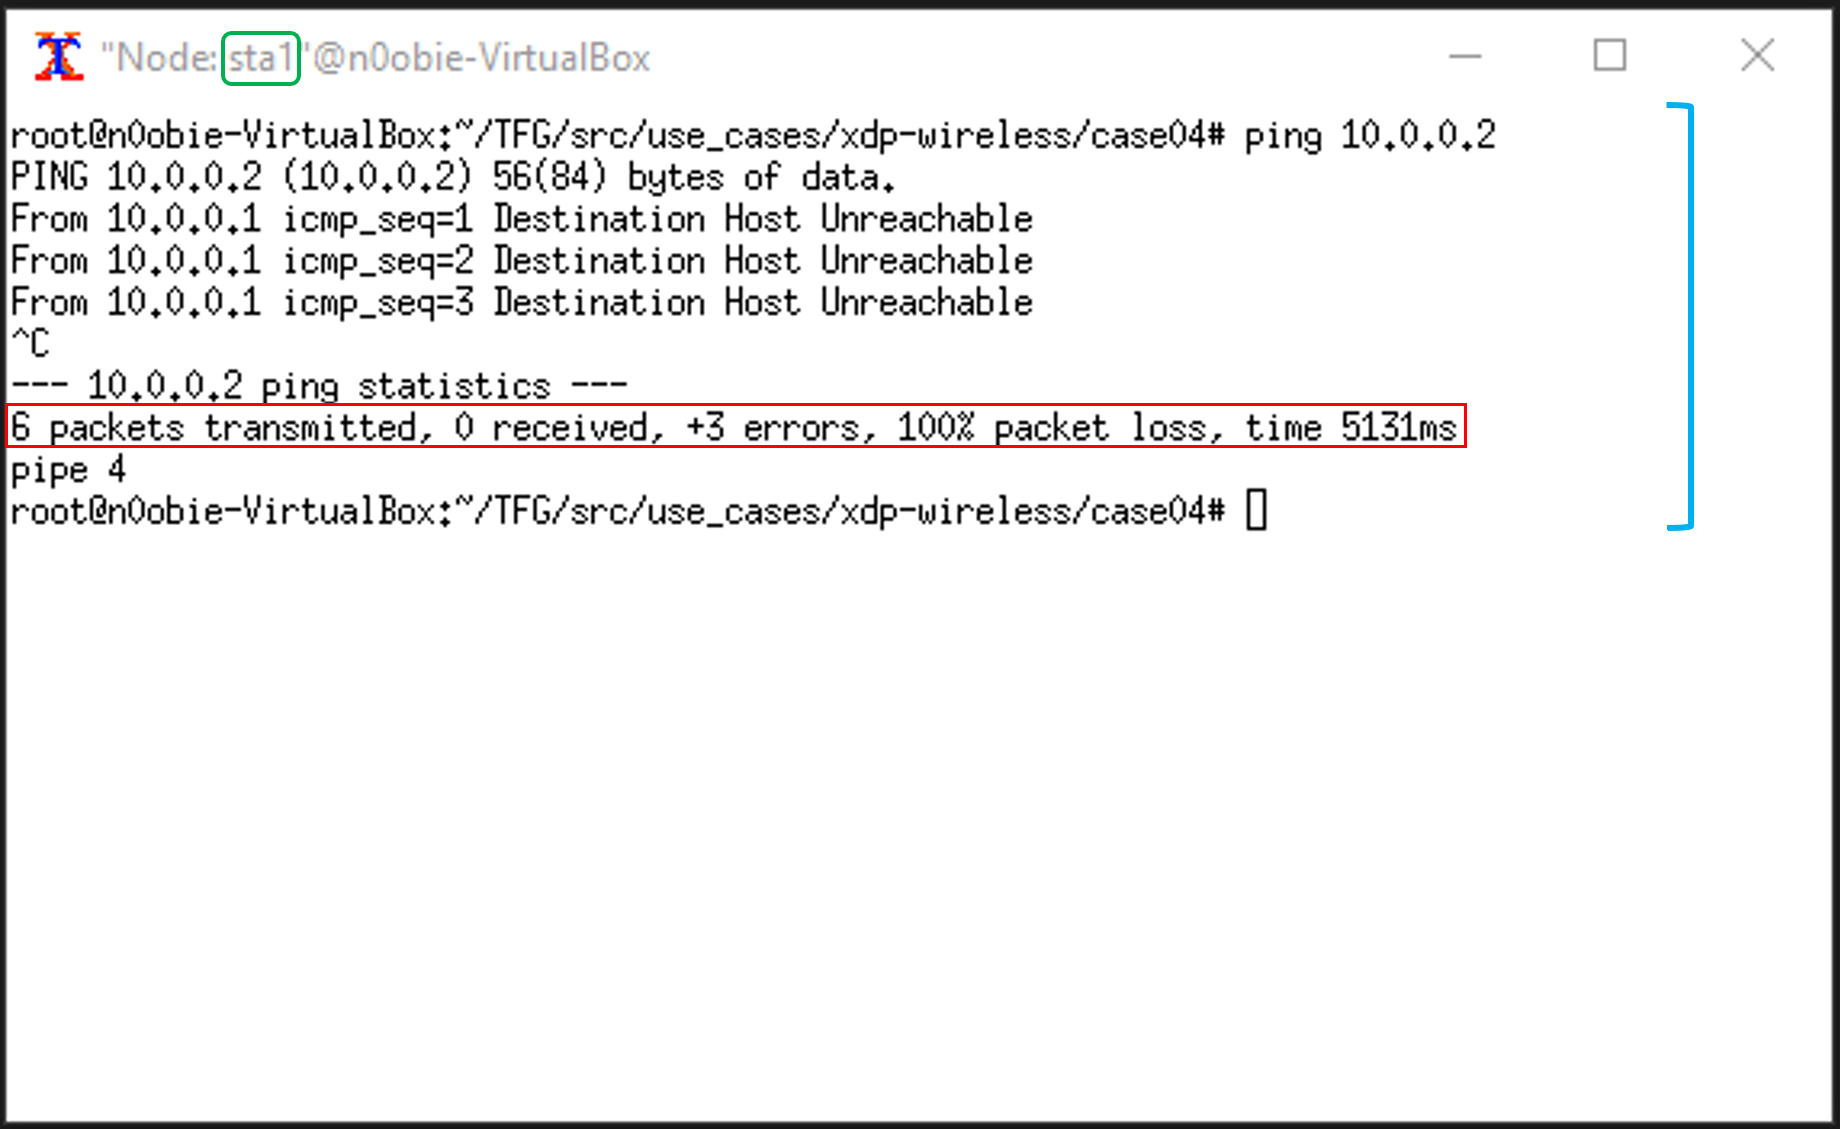
\includegraphics[width=10cm]{archivos/img/dev/xdp-wifi/case04/demo_case04_hard_1_edited.png}
    \caption{Ping Hardcoded forwarding del Case04 - XDP Wireless}
    \label{fig:case04_xdp_wifi_func1}
\end{figure}

% figura escenario
\begin{figure}[ht!]
    \centering
    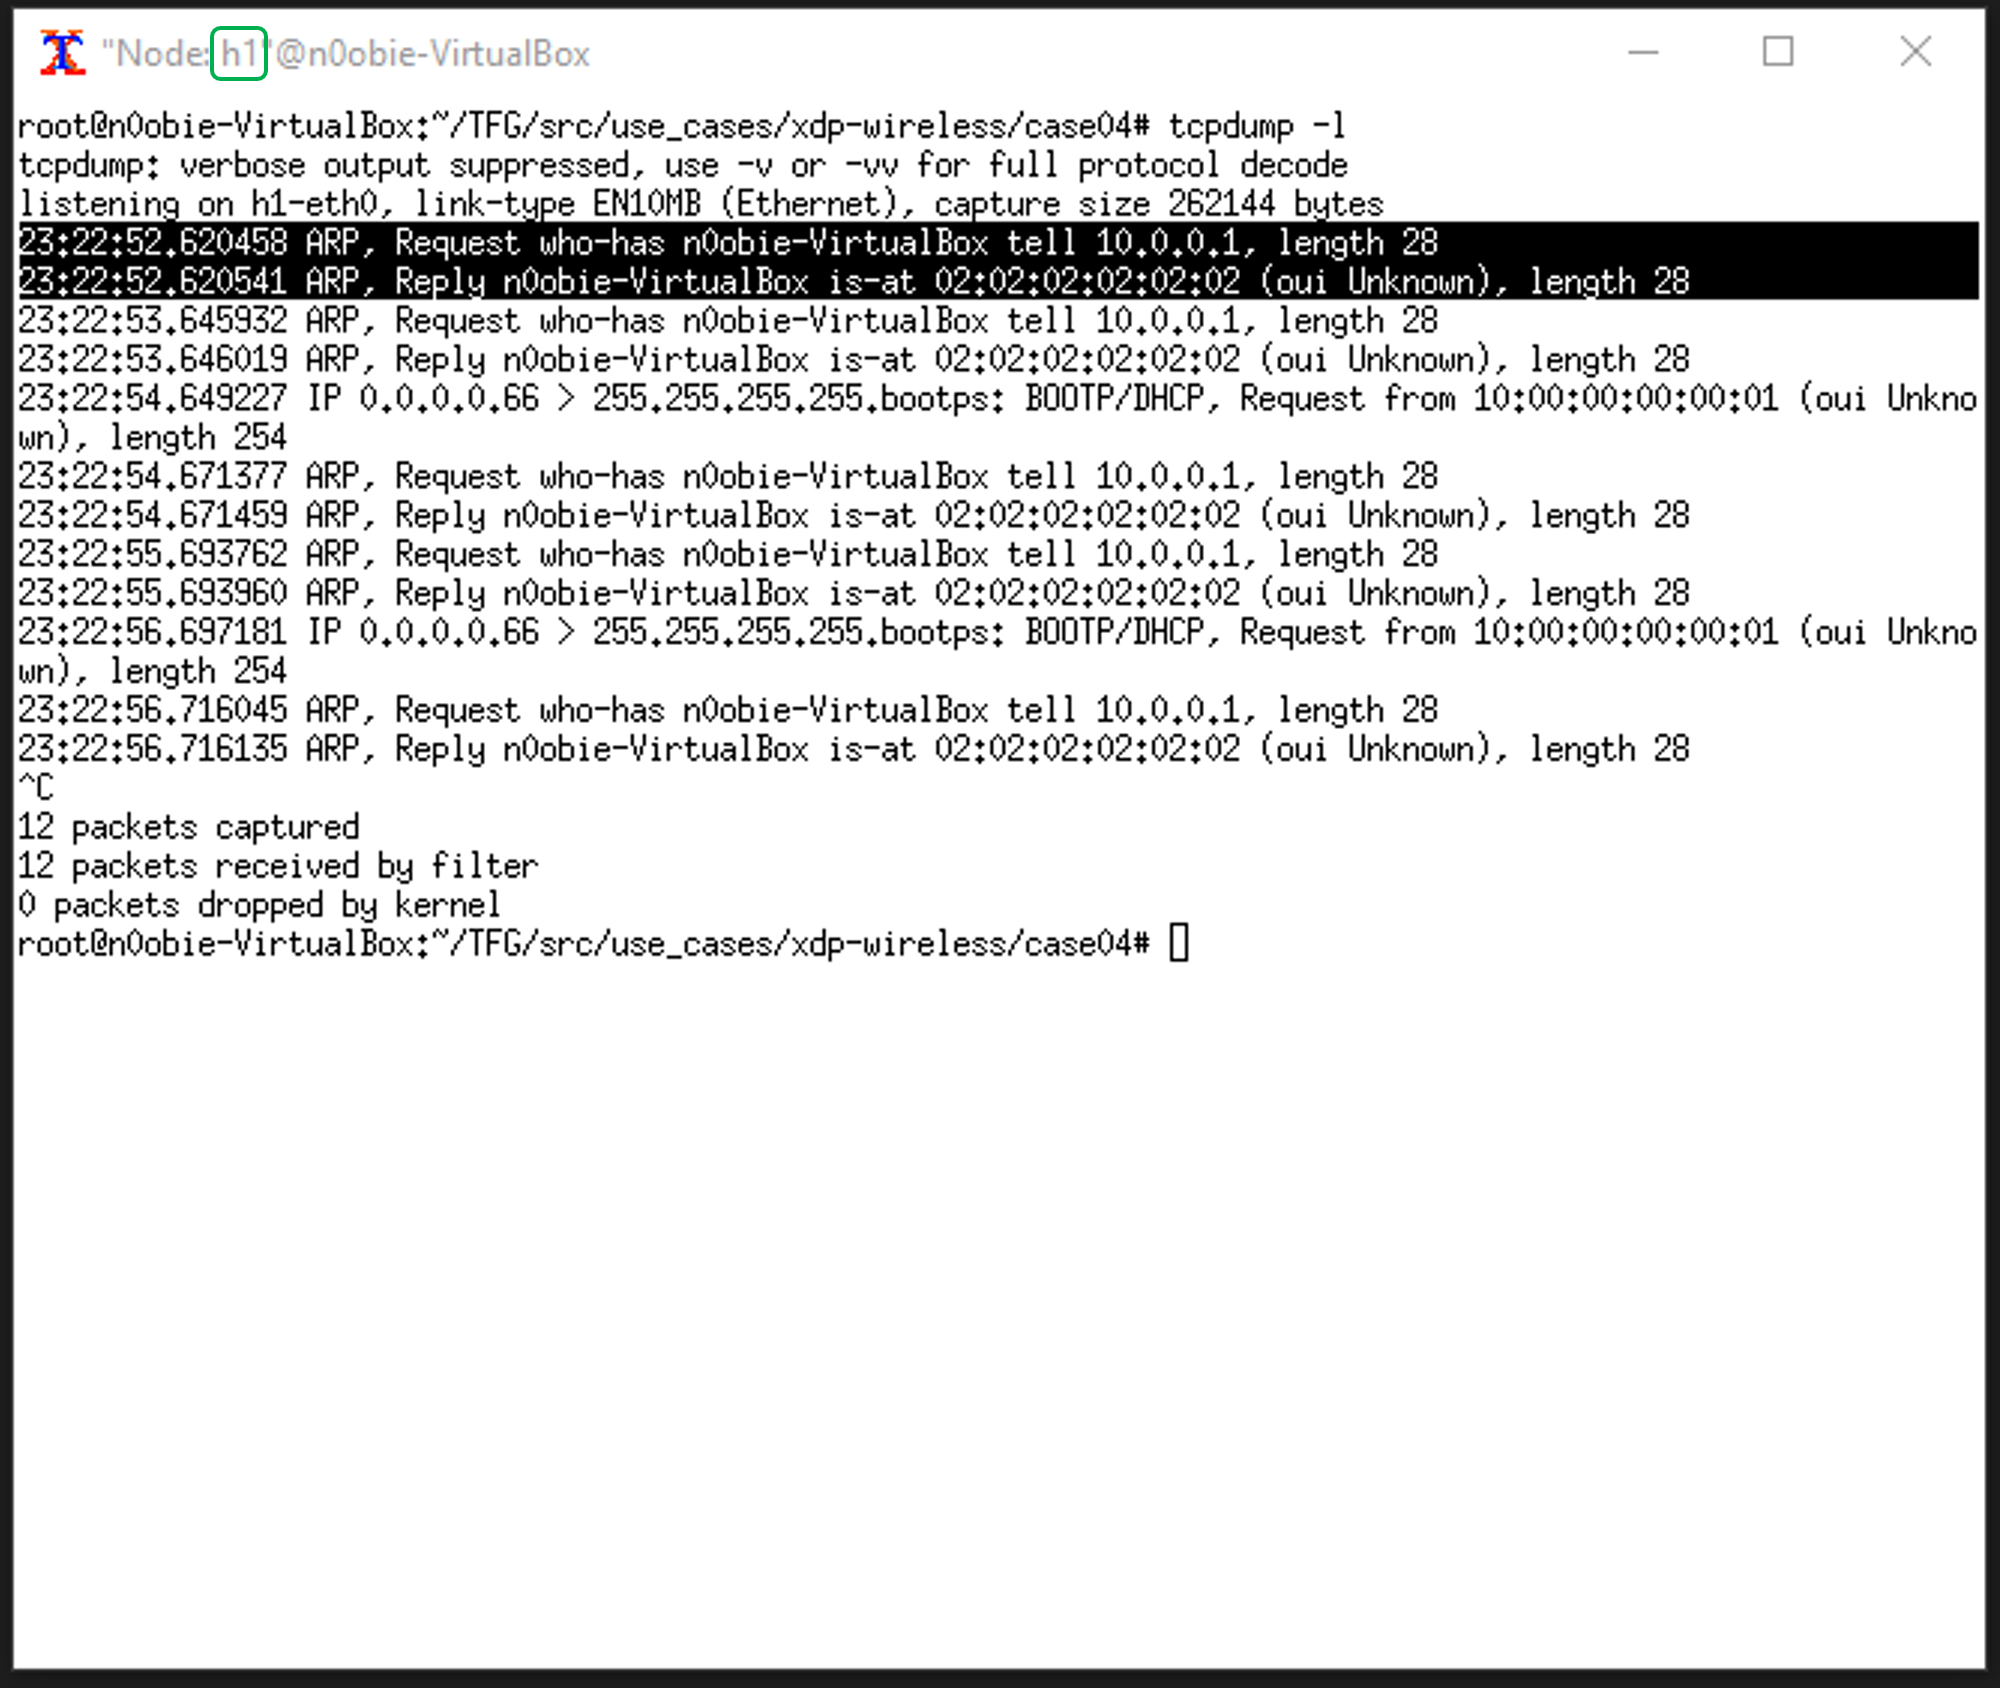
\includegraphics[width=10cm]{archivos/img/dev/xdp-wifi/case04/demo_case04_hard_2_Edited.png}
    \caption{Sniffer Hardcoded forwarding del Case04 - XDP Wireless}
    \label{fig:case04_xdp_wifi_func2}
\end{figure}

Se puede, de forma adicional, añadir la entrada ARP de forma estática a la \textit{Network Namespace} de la estación \textit{wireless} \texttt{sta1} pero el ping seguiría sin funcionar, ya que los paquetes \texttt{ECHO-Reply} asociados a los \texttt{ECHO-Request} recibidos nunca podrán llegar de vuelta a la estación \textit{wireless} \texttt{sta1}. En el siguiente escenario de forwarding se abordará esta carencia en la comunicación con un nuevo planteamiento para conseguir bidireccionalidad en la comunicación, a la par que escalabilidad.

%%%%%%%%%%%%%%%%%%%%%%%%%%%%%%%%%%%%%%%%%%%%%%%%%%%%%%%%%%%%%%%%%%%%%%%%%%%%%%%%%%%%
\subsubsection{Semi-Hardcoded forwarding (BPF maps)}
\label{xdp_wifi_case04_semihard}

La segunda forma de implementar el forwarding se denominará Semi-Hardcoded forwarding, como ya se comentó, la información irá hardcodeada, pero no en el propio programa \gls{xdp}, sino, en los mapas \gls{bpf}. El escenario levantado (Ver figura \ref{fig:case04_xdp_wifi_scenario2}), está compuesto de una estación wireless y un host, que corren dentro de su respectivas \textit{Network Namespaces}, y un punto de acceso corriendo un proceso de HostApd para comunicar las dos estaciones wireless entre sí. De forma adicional, y por consistencia del caso de uso, se ha decidido ejecutar dicho switch dentro de su propia \textit{Network Namespace} para que no haya lugar a dudas de que el forwarding se está realizando correctamente y no está habiendo \textit{by-passes} de ningún tipo. En este caso el forwarding se hará desde la interfaz \texttt{ap1-wlan1} hacia la interfaz \texttt{ap1-eth2} y viceversa.


% figura escenario
\begin{figure}[ht]
    \centering
    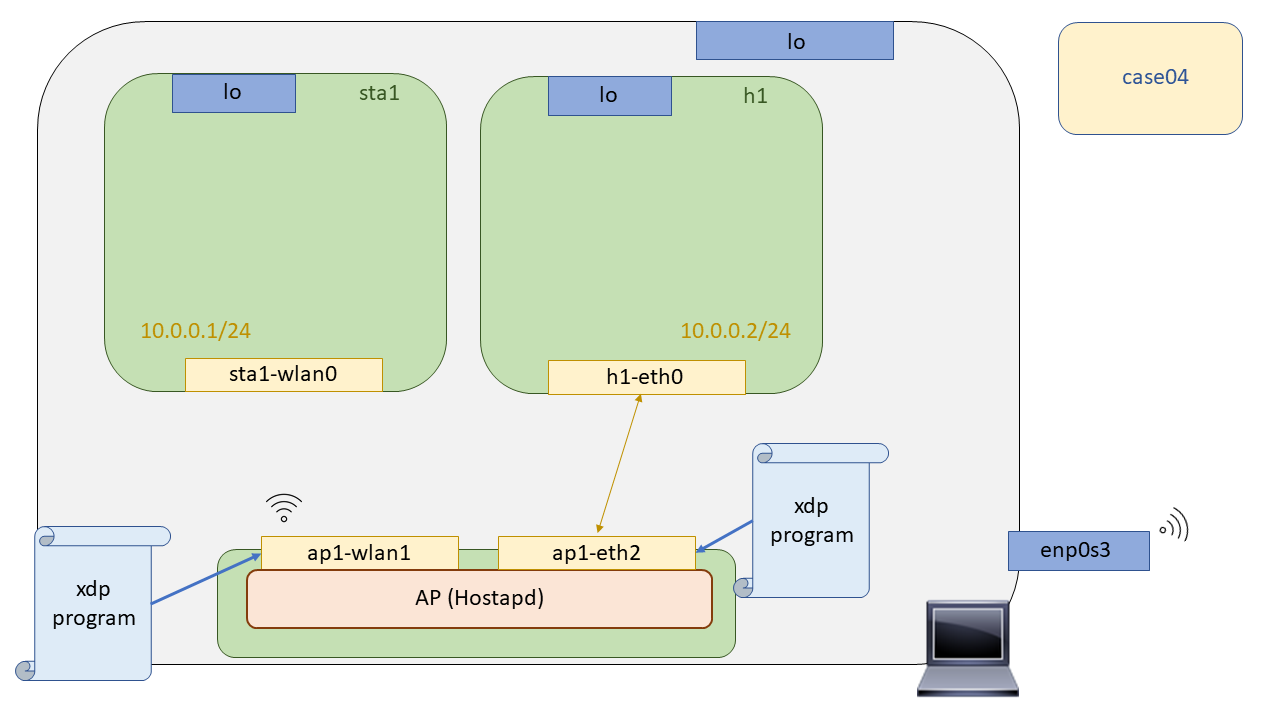
\includegraphics[width=16cm]{archivos/img/dev/xdp-wifi/case04/scenario_b.png}
    \caption{Escenario inalámbrico Semi-Hardcoded forwarding del Case04 - XDP Wireless}
    \label{fig:case04_xdp_wifi_scenario2}
\end{figure}


\vspace{0.5cm}
\textbf{Carga del programa XDP}\\
\par

Esta manera de hacer el forwarding no requiere de hardcodear datos en el propio programa XDP. En cambio, se usarán los mapas BPF como medio para guardar información de forwarding (ifindex y MACs destino) desde espacio de usuario, para que posteriormente el programa anclado en el Kernel sea capaz de leer los mapas, obtener la información de forwarding y realizarlo en base a la información percibida de los mapas BPF. Es importante señalar que los programas anclados previamente deben ser eliminados, por lo que una opción sería hacer un \textit{clean} del escenario haciendo uso del Makefile dado (\texttt{sudo make clean}) y empezar de nuevo. Por tanto, para anclar los programas \gls{xdp} se deberán seguir las indicaciones del bloque \ref{code:case04_xdp_wifi_load1}.

\begin{lstlisting}[language= bash, style=Consola, caption={Carga del programa XDP Semi-Hardcoded forwarding - Case04},label=code:case04_xdp_wifi_load2]
    # Lnazamos el script que levanta el escenario
    sudo python runenv.py
    
    # Anclamos el programa XDP en cada interfaz para conseguir un comunicación bidireccional 
    mininet-wifi> ap1 ./xdp_loader -d ap1-wlan1 -F --progsec xdp_case04_map -S
    mininet-wifi> ap1 ./xdp_loader -d ap1-eth2 -F --progsec xdp_case04_map -S
    
    # Almacenamos la información necesaria para realizar el forwarding y populamos los mapas BPF
    # con la información útil para llevar a cabo el forwarding en ambas direcciones.
    mininet-wifi> ap1 ./redirect.sh
\end{lstlisting}

\vspace{0.5cm}
\textbf{Comprobación del funcionamiento}\\
\par

La comprobación de funcionamiento de este programa puede ser llevada a cabo desde un extremo u otro debido a que, si todo funciona correctamente, existirá una comunicación bidireccional. Por lo que en este caso se harán las pruebas desde la estación wireless \texttt{sta1} hacia el host \texttt{h1}. 

\begin{lstlisting}[language= bash, style=Consola, caption={Comprobación del funcionamiento Semi-Hardcoded forwarding - Case04},label=code:case04_xdp_wifi_func2]
    # Hacemos un ping desde el h1 a la sta1, o al revés
    mininet-wifi> sta1 ping h1
    
    # Comprobamos con el recolector de estadísticas que se están produciendo XDP_REDIRECT
    mininet-wifi> ap1 sudo ./xdp_stats -d ap1-wlan1
\end{lstlisting}

% figura escenario
\begin{figure}[ht!]
    \centering
    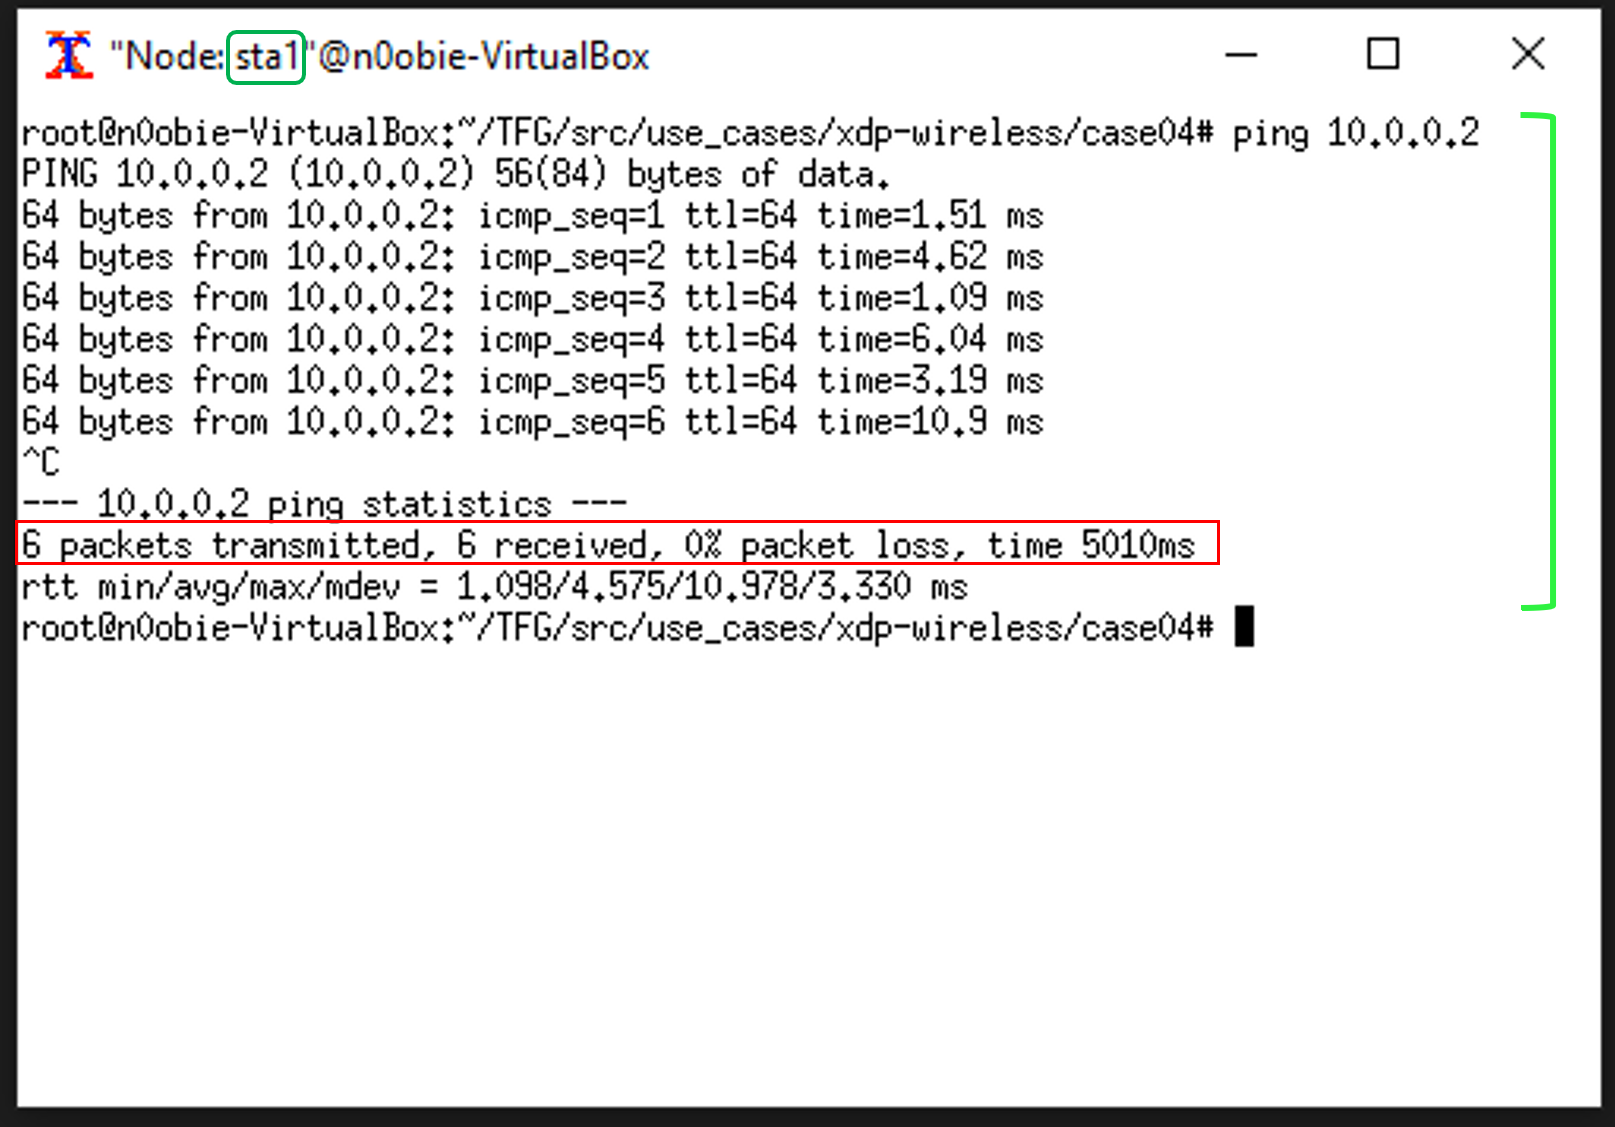
\includegraphics[width=9cm]{archivos/img/dev/xdp-wifi/case04/demo_case04_semihard_3_edited.png}
    \caption{Ping Semi-Hardcoded forwarding del Case04 - XDP Wireless}
    \label{fig:case04_xdp_wifi_func3}
\end{figure}

\vspace{0.5cm}

Como se puede apreciar en la figura \ref{fig:case04_xdp_wifi_func3}, hay perfecta conectividad, ya que el ping \fcolorbox{black}{green}{\rule{0pt}{2.5pt}\rule{2.5pt}{0pt}}\hspace{1mm} se ejecuta sin problemas entre la estación WiFi y el host, además los códigos de retorno \texttt{XDP\_REDIRECT} van aumentando (Ver figura \ref{fig:case04_xdp_wifi_func4}) siendo esto un indicador de que el programa efectivamente está llevando a cabo el forwarding.

\newpage

% figura escenario
\begin{figure}[ht!]
    \centering
    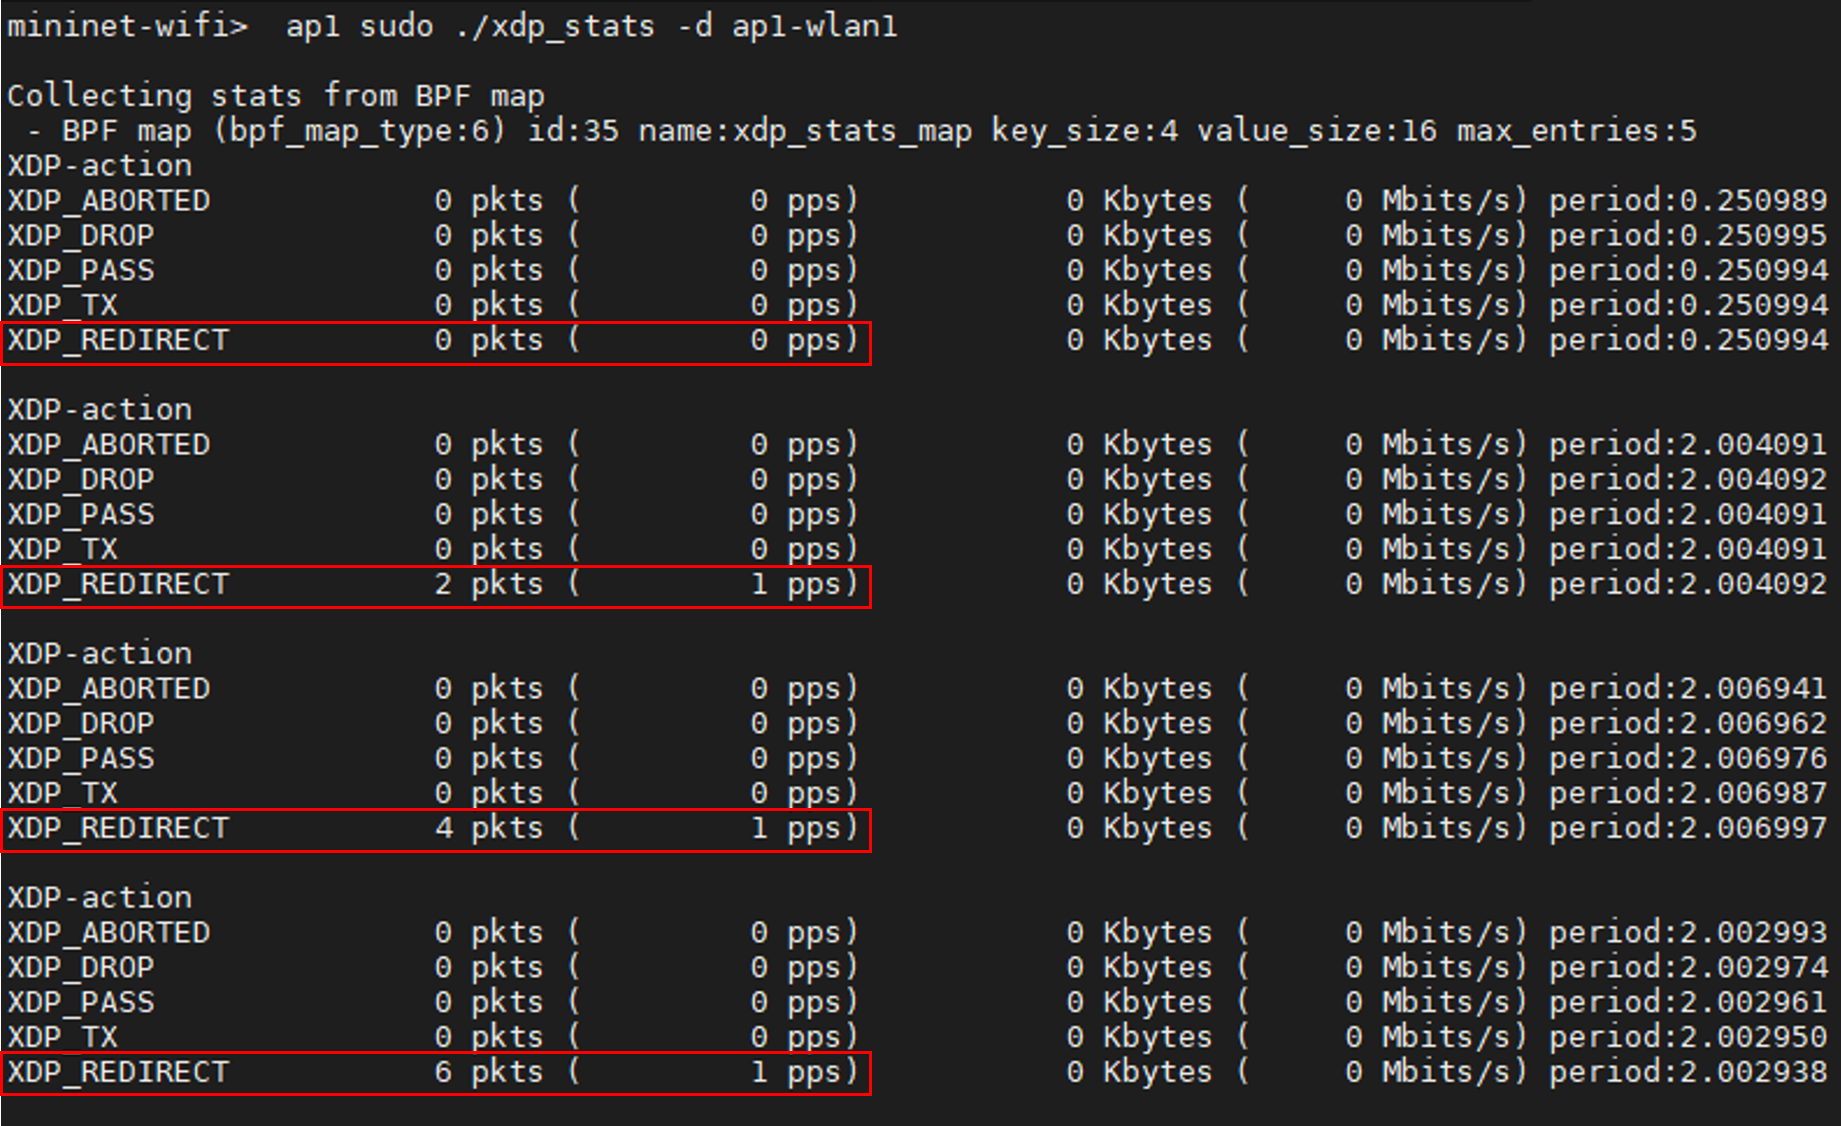
\includegraphics[width=15.5cm]{archivos/img/dev/xdp-wifi/case04/demo_case04_semihard_2_edited.png}
    \caption{Stats Semi-Hardcoded forwarding del Case04 - XDP Wireless}
    \label{fig:case04_xdp_wifi_func4}
\end{figure}

%%%%%%%%%%%%%%%%%%%%%%%%%%%%%%%%%%%%%%%%%%%%%%%%%%%%%%%%%%%%%%%%%%%%%%%%%%%%%%%%%%%%
\subsubsection{Forwarding auto (Kernel FIBs)}
\label{xdp_wifi_case04_auto}

En esta última alternativa, no se pudo replicar  debido a que existía una incompatibilidad del escenario propuesto con ese tipo de forwarding. Esto debe a que el forwarding automático se alimentaba de las rutas de la FIB del Kernel, pero al estar aislado el punto de acceso en su propia \textit{Network Namespace}, no era capaz de obtener dicha información.